%!TEX root = ../../main.tex

\chapter{EDRICO (Educational DHBW RISC-V Core)}

The Proposed Processor design named EDRICO implements a basic RV32I
instruction set architecture. Besides the mandatory “Zicsr” extension no other
instruction set extensions are implemented. To keep the implementation simple and
straight-forward only one privilege mode (Machine-mode) is implemented. This mode
allows full access to the processor and peripherals. Future Versions could be
extended to implement S-Mode and U-Mode.
The core is a simple \acf{SISD} processor without any pipeline or even cache. The basic
instruction cycle of fetch, decode, execute, store is performed for every instruction
one at a time.\\
Figure \ref{fig:edricooverview} shows the full overview of the processor design:

\begin{figure}[H]
	\centering
	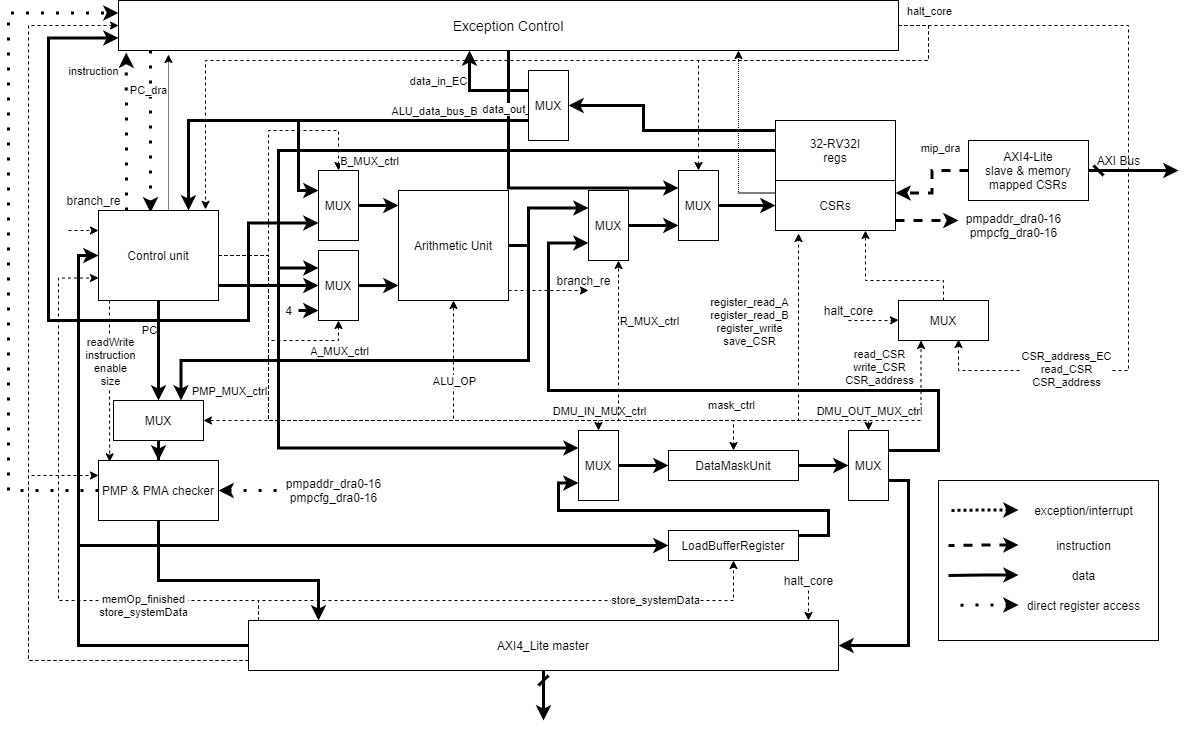
\includegraphics[width=150mm,scale=0.5]{datapath_EDRICO}
	\caption{EDRICO Overview}
	\label{fig:edricooverview}
\end{figure}

Its main components are the Exception Control, Control Unit, Arithmetic Unit,
Register Files, PMP \& PMA checker and the AXI4 Interfaces.
Each one of the components will be described in more detail in the following section.

\section{Control Unit}
The \ac{CU} is the heart of the processor and controls the other parts of the processor depending on the input instruction. The CU is responsible for fetching instructions from the instruction memory, decode the bitstream and set the respective control signals for the other processor components. Due to the complexity of the CU, there are several sub-modules which together form the overall CU.
A general overview of the CU architecture is displayed in Figure \ref{fig:cuarchitecture}. 

\begin{figure}[H]
	\centering
	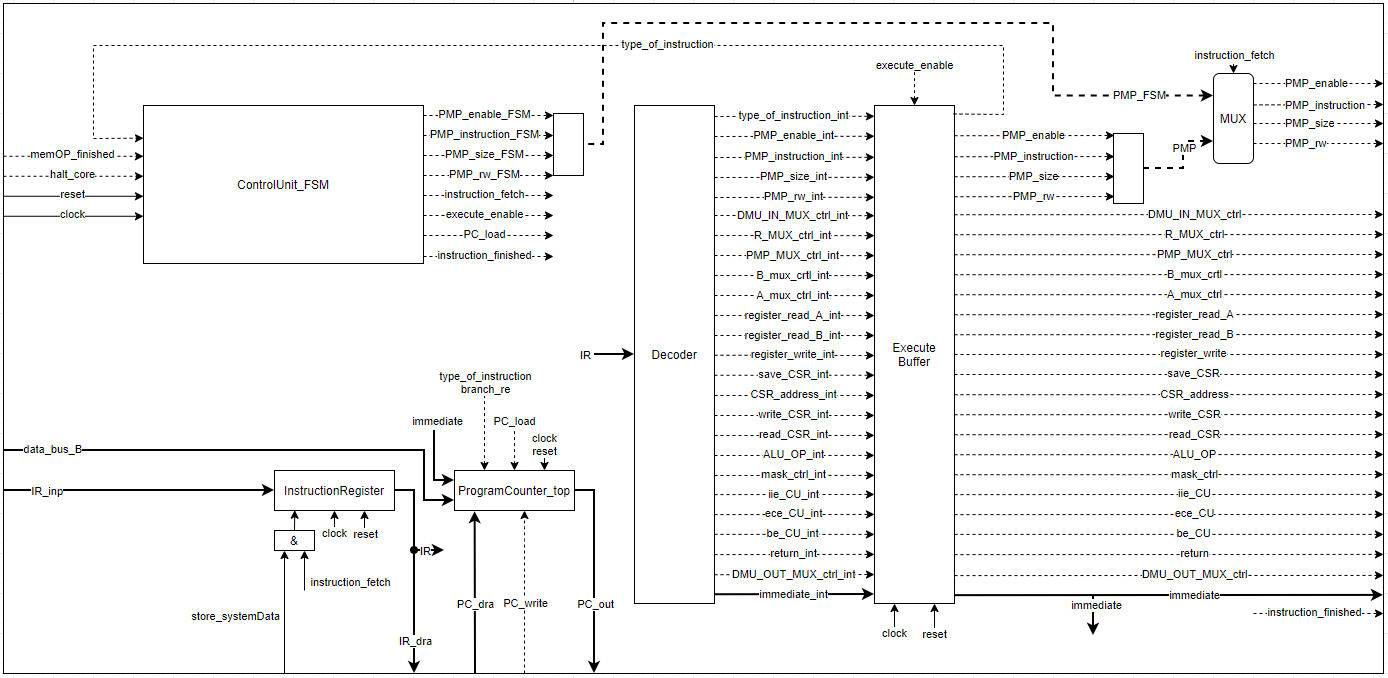
\includegraphics[width=\textwidth]{CU_architecture}
	\caption{Control Unit Architecture}
	\label{fig:cuarchitecture}
\end{figure}

To describe the functionality of the CU in more detail, every sub-module will be described closely.\\
Since the Control Unit is responsible for the whole processor, it is important to have a persistent and stable procedure for every instruction that shall be executed. The Control Unit \ac{FSM} is responsible for the correct clock timings which is important due to memory operations and the execution time of the other processor parts. The states and conditions of the FSM are displayed in Figure \ref{fig:cufsm}. 

\begin{figure}[H]
	\centering
	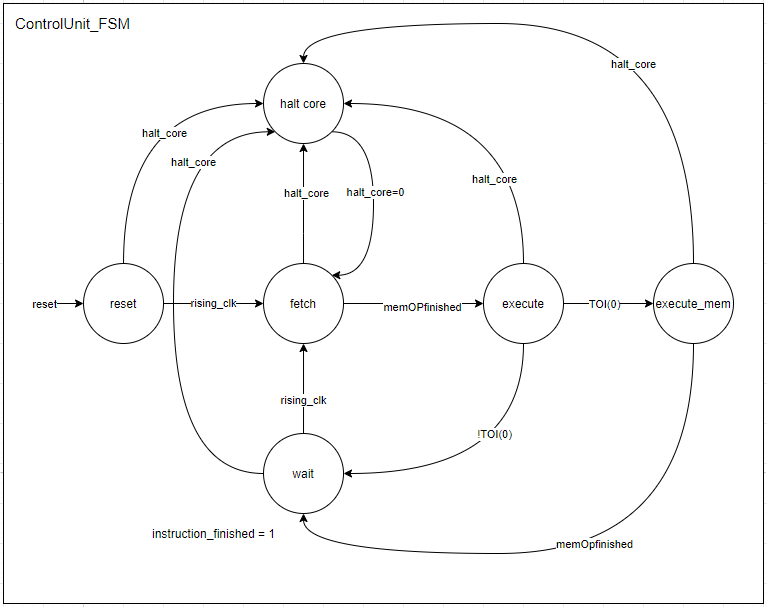
\includegraphics[width=\textwidth]{CU_FSM}
	\caption{Control Unit FSM overview}
	\label{fig:cufsm}
\end{figure}

Table \ref{tableFSM} shows a more detailed overview of the clock cycles and the corresponding actions and states:\\

\begin{table}[h]
\resizebox{\textwidth}{!}{
	\begin{tabular}{|c|c|l|l|}
		\hline
		\textbf{ClockCycle} & \textbf{Edge} & \textbf{Action} & \textbf{Signal} \\
		\hline
		1 & rising & pass the PC and enable PMP \& PMA checker with respective information &  \\
		\hline
		& falling & N/A &  \\
		\hline
		4 & rising & data is ready in instruction register - switch to execute state & \textit{memOPfinished} \& \textit{store\_systemData} is high \\
		\hline
		5 & rising & execution is started - if memory operation wait for another \textit{memOPfinished} flag, otherwise wait & \textit{execute\_enable} \\
		\hline
		x & rising & during memory operation: data loaded to buffer \textbackslash store transfer finished $\rightarrow$ wait state & \textit{memOPfinished} \& \textit{store\_systemData} is high \\
		\hline
		& falling & if load: store data form buffer to specified location &  \\
		\hline
		6 / x+1 & rising & go to \textit{fetch\_state} &  \\
		\hline
	\end{tabular}}
\caption{Timing of FSM}
\label{tableFSM}
\end{table}

During an execution cycle, the FSM controls the rest of the CU consisting of memory, decoding unit, PC control and the different multiplexers. To understand what the purpose of the different signals are, the other components of the Control Unit are described in the following sections.


